%!TEX TS-options = -shell-escape
\documentclass[oribibl]{llncs}
\pagestyle{headings} %page numbers
\usepackage{makeidx}  % allows for indexgeneration

\usepackage[utf8]{inputenc}
\usepackage{pdfpages}

% \usepackage[nottoc,numbib]{tocbibind}
% \usepackage[center]{caption}

\usepackage{float}

\usepackage{enumitem}
\usepackage[T1]{fontenc} % Fixed missing font warning for \maketitle
%\usepackage[margin=1.5in]{geometry}
\usepackage{url}
\usepackage[multiple]{footmisc} % DOUBLE FOOTNOTES ACROSS THE SKY
\renewcommand{\footnotemargin}{3.99pt}

% %% to make urls look better in bibliography
% \makeatletter
% \def\url@leostyle{%
%   \@ifundefined{selectfont}{\def\UrlFont{\sf}}{\def\UrlFont{\small\ttfamily}}}
% \makeatother
% %% Now actually use the newly defined style.
% \urlstyle{leo}

\bibliographystyle{plain}



\begin{document}

% insert the table of contents if want, it is not required
% llncs says: "If you are the author of a single contribution you
% normally have no running heads and no table of contents."
% \tableofcontents

\mainmatter              % start of the contributionsmainmatter
\title{Textual Editing of Partial IFC Model}

\author{Nicolai Dahl Blicher-Petersen \and Christian Harrington \and
Thomas Hallier Didriksen \and Sune Alkærsig \and Anders Høst Kjærgaard\\
\email{\{ndbl, cnha, thdi, sual, ahkj\}@itu.dk}}

% Do we want to show our emails?
\institute{IT University of Copenhagen, Rued Langgaards Vej 7, 2300 Copenhagen S, Denmark}


\maketitle              % typeset the title of the contribution

\begin{abstract}
Industry Foundation Classes (IFC) is an ISO standard used for modelling various physical and functional aspects of a building. IFC models are often large and complex, so a key challenge is: how can work be carried out on e.g. plumbing, heating, or electrical wiring independently without introducing inconsistencies. This paper describes a prototype solution that eases cross-disciplinary work, by allowing model evolution and resolution of inconsistencies on a small subset of a large IFC model. The model-driven methodology is used to achieve a generally applicable and flexible solution, usable in various domains. In this paper we demonstrate an open source prototype handling a common industry problem that specifically makes it possible to edit pipes, walls, and openings in walls.

\keywords{IFC, BIM, EMF, DSL, model-driven development, model transformation, Xtext, Xtend, BIMServer}
\end{abstract}


%!TEX root = ./report.tex


% Slides:
% - General statement introducing the area; You can most likely start with the first paragraph from your project description and evolve it.
% - Explanation of the specific problem and why do we care about the problem.
% - Explanation of your solution, and how it improves on the work by others. Relation to related work can be very brief, given that you have a separate extensive section devoted to this.
%  -A hint on how the solution was evaluated and what was the outcome of this evaluation.
%  -A summary (a “map”) of how the paper is organized.

\pagenumbering{arabic}
\setcounter{page}{1}
\section{Introduction}
Building Information Modelling (BIM) is the process of modelling various physical and functional aspects of a building\cite{clar:eke}. Currently, many BIM software products exist. These let a user model and analyze the many interactions between different parts of a building. Many of these software products use common file formats for modeling buildings, such as Industry Foundation Classes (IFC) or Green Building XML (gbXML). These formats were invented to help improve interoperability between different software packages in different domains, and as such cover many different systems. These formats have become widely used standards.

Reading and writing a huge, complex XML document, like the ones produced by BIM products, by hand is unfeasible. It’s desirable to be able to work with aspects of a model (such as heating, or electrical wiring) independently.(TODO insert reference) In this paper we present a setup, demonstrating that such projectional editing is feasible.

Introduction still missing:
- Explanation of your solution, and how it improves on the work by others. Relation to related work can be very brief, given that you have a separate extensive section devoted to this.
- A hint on how the solution was evaluated and what was the outcome of this evaluation (may be omitted in out case)
- A summary (a map) of how the paper is organized.



Outline:
Feasibility study of whether it is possible to do projectional editing on IFC.

What were the challenges?
- Saving the subset back to the server after editing. Synchronization problem
- Using MPS: it is not a freetext editor. We would want to improve on this later. XText is not flexible enough for this purpose.

Important to mention:
- Ideally this would be a visual editor, but in order to make the project feasible our prototype will use textual syntax - a DSL.

Perhaps as conclusion (from problem statement):
- This DSL, along with the generated tools, will provide a human readable representation of these building models, and can serve as a building block for Energy Futures projects to come. Additionally, the experience gained by building this DSL, will contribute to the overall knowledge of this area for the Energy Futures research initiative.
%!TEX root = ./report.tex
\section{Background}
\label{sec:background}
In this section we provide an overview of BIM and some of the challenges in working with IFC. Lastly we discuss relevant technologies to be used for providing a solution.
\subsection{Building Information Modeling}

\label{sec:building_information_modeling}
(FIXME Den første del her er allerede skrevet i starten af Introduction)BIM is a method that through generating digital representations, model physical constructions. The resulting model is a shared knowledge base that can be used in all the stages of a building project, ranging from the earliest conceptual stages, construction, to day to day management and even demolition. BIM extends traditional building design from two dimensional drawings and three dimensional physical models, to also include aspects like time, cost, manning and process into the model. This makes BIM very attractive to modern building constructors, as it not only eases up the communication between the many different parts involved in a building, but also allows for early planning in terms of time- and energy consumption.

To support the flexibility required in BIM, it has to be represented in a format that gives rise to interoperability. And since building projects involve many different contributers from different domains, it has to be adoptable by many different software applications\,\cite{quteprints37725}. In effect, most software applications in BIM projects, will only work on a subset of the model.
\subsection{Industry Foundation Classes}
IFC is commonly used for BIM and is mandatory for new public buildings in Denmark.\footnote{Regulations for buildings built by the Danish state \url{https://www.retsinformation.dk/forms/R0710.aspx?id=134884}}. Its goal is to facilitate interoperability between different software platforms. It does this through an object-based data model. There are two main file formats of IFC. The first is a EXPRESS based format, IFC-EXPRESS (ISO-10303-21), with the file extension ".ifc". The other is based on XML, and called ifcXML (ISO-10303-28), with the file extension ".ifcxml". The EXPRESS based format is the most commonly used due to its relative compact size, while still being readable.

One of the main challenges when working with IFC is the size of it. The entity model contains more than six hundred entities organized in an object-based inheritance hierarchy. Entities can be both tangible elements, such as an IfcWall, but also abstract entities like IfcAxis2Placement3D describing the location and orientation of another IFC entity. On the highest level of abstraction, IFC defines two categories of elements, being rooted and unrooted elements. Unrooted elements do not have an identity and only exist if referred to by other elements. Rooted elements have a unique global identity (GUID) and are subdivided further into three groups: IfcObjectDefinitions are abstract definitions of anything from tangible elements to definitions of work processes, IfcRelations are relations between other objects, and IfcPropertyDefinitions are properties of other objects. The model is further subdivided multiple times.

IFC is not the only file format used for BIM. Another prominent format is Green Building XML (gbXML) which also focuses on interoperability, and as the name suggests, lowering energy consumption. Although gbXML seems well evolved and flexible, for our purpose, IFC seems to be the best suited and also the most widely adopted.

\subsection{Eclipse Modeling Framework and Ecore}
The Eclipse Modeling Framework is a modeling framework and code generation facility for building tools and other applications based on a structured data model\footnote{The EMF project page can be found at \url{http://www.eclipse.org/modeling/emf/}}. EMF is capable of producing a Java object graph from a model instance described in XMI. For meta modeling this instance EMF includes Ecore. Ecore is a meta modeling language allowing the user to describe and build meta models for their domain. Furthermore EMF has several transformation tools, enabling transformation from either one Ecore model to another or from Ecore model directly to a textual format.

%!TEX root = ./report.tex
\section{Problem Analysis and Requirements}
In the following section we will analyse the presented problem, and discuss a set of requirements for a solution that is capable of editing a partial IFC model within a specific domain. This list should be thought of as a guideline for how this problem should ideally be approached, if the project results were to be replicated. The list is formed by theoretical knowledge, as well as experience gained through the course of the development of the solution.

\subsection{Problem Analysis}
\label{subsec:problem_analysis}
The separation of the construction model and plumbing model causes it to be difficult to keep consistency between the two. In this project we will focus on how IfcFlowSegments (e.g. a pipe), IfcWallStandardCases (a regular wall) and an IFCOpeningElement (a hole in a regular wall) interact. Kaj Jørgensen mentions that a possible solution to the problem is to allow the building service engineer to create a message with precise information about required holes, or openings, for the pipes\,\cite{jorgensen12}. This message should then be handed to the construction engineer, such that he is able to verify that these are properly placed. A part of doing this is facilitating a transformation of IFC into a subset of the domain, where it is easy for the user to make changes to this subset, and reflect these changes back to the original IFC. As such, the primary goal of the solution is to enable the user to work on a subset of the IFC model involving pipes, openings, and walls. In Figure \ref{fig:ifcheirachy} a graphical representation of this subset is presented, excluding relational objects, such as IfcRelVoidsElement.

\begin{figure}[t]
    \centering
        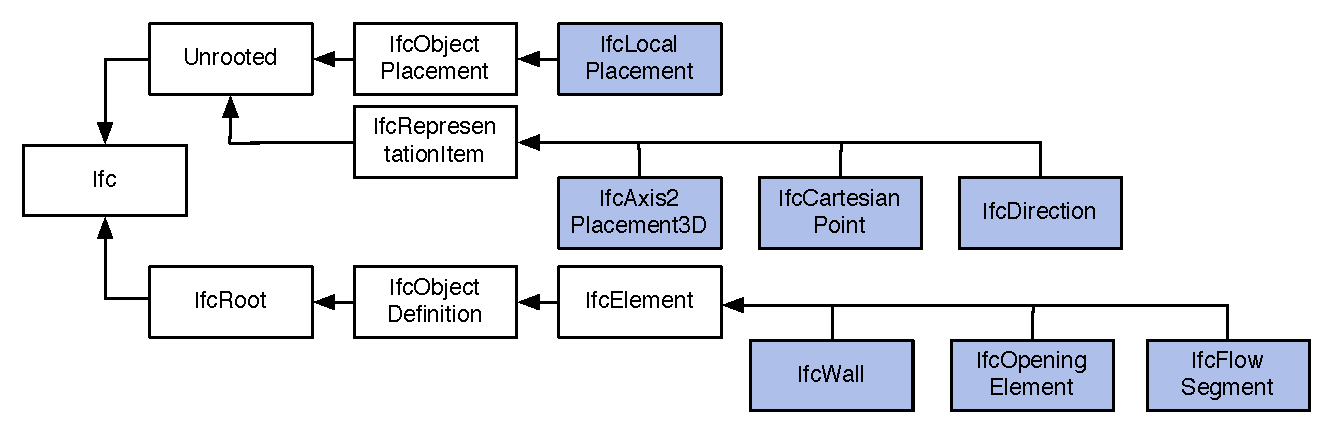
\includegraphics[width=110mm]{images/IfcHeirachy.pdf}
    \caption{A graphical representation of the subset used, excluding relational objects for the sake of simplification. The objects of the chosen subdomain are highlighted in blue.}
    \label{fig:ifcheirachy}
\end{figure}

\subsection{Requirements}
\label{subsec:requirements}
\paragraph{Working with a Partial Model}
With the aforementioned complexities and challenges of IFC in mind, a primary focus is to be able to extract a well-specified subset of an IFC model. It is desirable to have an architecture that separates this concern from the rest of the workflow into one component and extracts the partial model that we are interested in. Reversely, the problem of re-inserting this partial model should also be implemented as a modular workflow component. This allows for easy reuse of the module and makes the correctness of the extraction process verifiable.

Furthermore, a clear domain definition is needed to implement and verify the extraction process. Achieving this in a concise but generic way turns out not to be entirely trivial. An evolving standard for this kind of specification is Model View Definitions(MVD)\,\cite{nour08}, which is a precise but extensive definition allowing fine-grained IFC subset specification in XML. buildingSMART, a non profit organization supporting open source BIM software, propagates MVD as their standard.\footnote{buildingSMART, Model View Definition, \url{http://buildingsmart.com/standards/mvd}} Nour discusses this and other challenges when working with partial editing on IFC\,\cite{nour08}. It was not possible for this project to obtain the product of Nour's project, and developing a similar product, capable of genericly extracting a subset of IFC based on and MVD, was deemed out of scope. Furthermore, defining a partial model with MVD is in itself a complicated task and for purposes of designing a single experimental DSL with only a few IFC classes a more informal definition of the domain is preferable to simplify the development process.

\paragraph{Correct Meta Model}
When loading an IFC building instance from EXPRESS or ifcXML to Ecore it is vital for the solution that the IFC meta model is in fact correct. This point may at first seem trivial but in our experience a correct EMF meta model that reflects the actual IFC standard is difficult to obtain, especially one that comes with a proper serializer/deserialiser converting from either EXPRESS or ifcXML to the corresponding Ecore instance. The difficulty lies in the fact that across existing implementations, it is not at all consistent how models are treated, so one must be aware of any inconsistencies in the meta model\,\cite[pp. 4]{quteprints37725}. %FIXME: 

\paragraph{Valid Model Transformations}
An ideal solution would produce model transformations that are verifiable and correct. By verifiable, we refer to being able to trace that transformations actually occur in the way that we require. By correct, we primarily refer to not corrupting any model structure during a transformation, but also to not breaking any constraints in the domains. However, with the complexity of IFC in mind, we will relax the requirement to not breaking any constraints. As such, the ideal solution would show that making a valid model to model trasformation between and IFC partial model and a Pipes model is feasible.

\paragraph{A Simple DSL}
When all these technical features have been accounted for the solution still needs a simple DSL. Key to a non-experimental solution is that it displays a part of the complex source domain in a simple, manageable way.  This being a feasibility study only the inclusion of a DSL as a proof of concept, and not the syntax or usability of this, is relevant. One could imagine that a future end product would indeed be visual instead of textual.

When implemented, a simple DSL will demonstrate that the partial model editing is feasible for any subdomain of IFC. In other words the implementation will show how a small but significant target domain, like the position of a pipe and a hole in a wall, can be managed separate from the main model. Therefore, to support extensibility and reusability, it should be built with wide-spread tools like EMF and Xtext.

\paragraph{Structural Editing}
A meaningful scope of what should be possible to do with the DSL, is the ability to edit existing values, say the position of a pipe, and more importantly, the ability to remove or add elements. The latter should be possible to resemble a real-world use case scenario, and the solution should be able to do this, of course, without corrupting the IFC instance.
\paragraph{}
This concludes the list of desirable features, but please note that it is only a core selection and that one could imagine many extensions to it. Some of these will be discussed in Section \ref{sec:plan_for_future_projects} as an idea for a future project. 


%!TEX root = ./report.tex
\section{Solution}
The final product combines several technologies to attain an extendable solution with two reusable Xtend client side workflows at its core. The setup allows the user to edit a subset of IFC in a generated Eclipse editor in between the two workflows. The main model is stored on a BIMServer for merging, versioning and extensibility purposes, as this section will further explain.

\subsection{Server Side}
The overall workflow of the end product is depicted in figure \ref{fig:overall_product_workflow}. As described in (TODO reference Kan Jørgensens workflow document) a construction model and a plumbing model are combined into one single model that needs to be verified for consistency. So called openings, i.e. holes in walls and floors need to be in place where the plumbing model describes flow segments to be installed. The merging of these models is executed on the BIMServer by the user as the first step of the workflow. When completed the client side of the end product allows the user to edit and add elements to the subset of the model.

\begin{figure}[htbp]
    \centering
        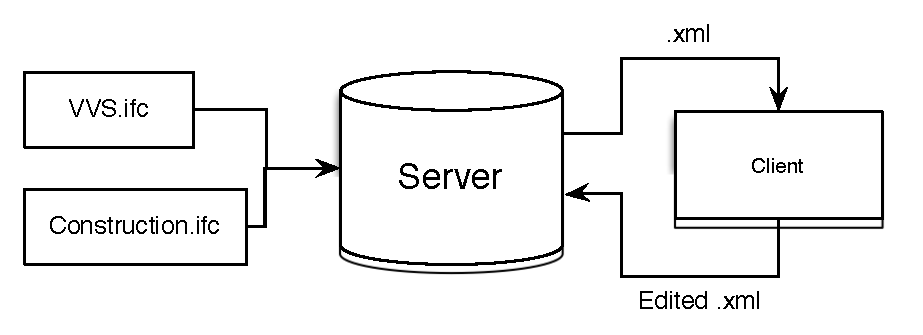
\includegraphics[width=120mm]{images/CompleteWorkflow.pdf}
    \caption{Overall Product Workflow}
    \label{fig:overall_product_workflow}
\end{figure}

We let a BIMServer handle the merging of models. Many tools exist for this job, but the special advantage of the BIMServer is that it also provides version control, conversion tools allowing the user to retrieve the saved building in other formats as well as Java client library. Especially the last feature is important for automating the workflow, as it allows for programatic server communication.

\subsection{Client Side}
Figure \ref{fig:IFC2PipesWorkflow} shows the IFC to Pipes workflow retrieving an IFC model from the BIMServer as XML, processing it to the corresponding java object graph, extracting the pipes and opening elements and converting these to an editable DSL instance, which is in turn saved to disk as an XMI file. The XML file loaded from the server is saved to the local disk for use by the second workflow explained below.

\begin{figure}[htbp]
    \centering
        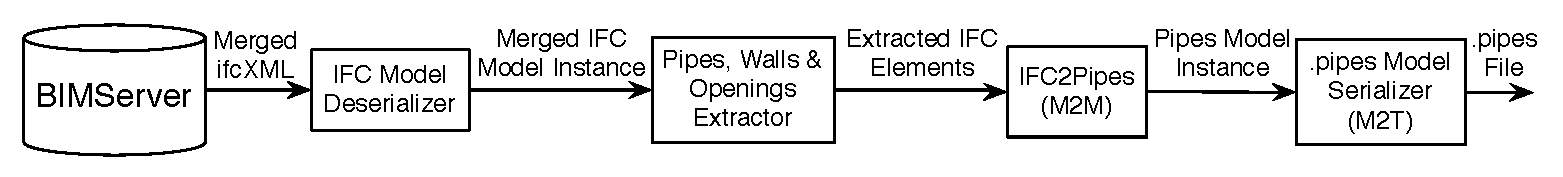
\includegraphics[width=120mm]{images/IFC2Pipes.pdf}
    \caption{IFC to Pipes DSL workflow}
    \label{fig:IFC2PipesWorkflow}
\end{figure}

The extraction process where relevant IFC elements are collected from the main model for conversion is implemented by a simple filtering mechanism extracting the pipes and opening elements. The real work of the IFC to Pipes workflow is done when this extract is converted to the corresponding Pipes DSL instance by utilizing the model to model transformation capabilities of the Xtend language. Each of the possible object occurences has a transformation rule specified here, making the conversion possible.
\paragraph{}
The second client side Xtend workflow, Pipes to IFC, is depicted on Figure \ref{fig:Pipes2IFCWorkflow}, where the user-edited XMI file is loaded into a Main Model Updater workflow module together with the non-updated extracted instance of the main model. Notice how the extraction is loaded in using the same workflow modules as in the first workflow, except the XML file is not fetched from the server but from the local disk. This makes for an easier update process in the Main Model Updater as the extracted instance is guaranteed not to have changed while the user was editing the XMI file. After the main model instance has been updated to reflect the users changes it is converted to XML and this new file is saved back to the BIMServer.

\begin{figure}[htbp]
    \centering
        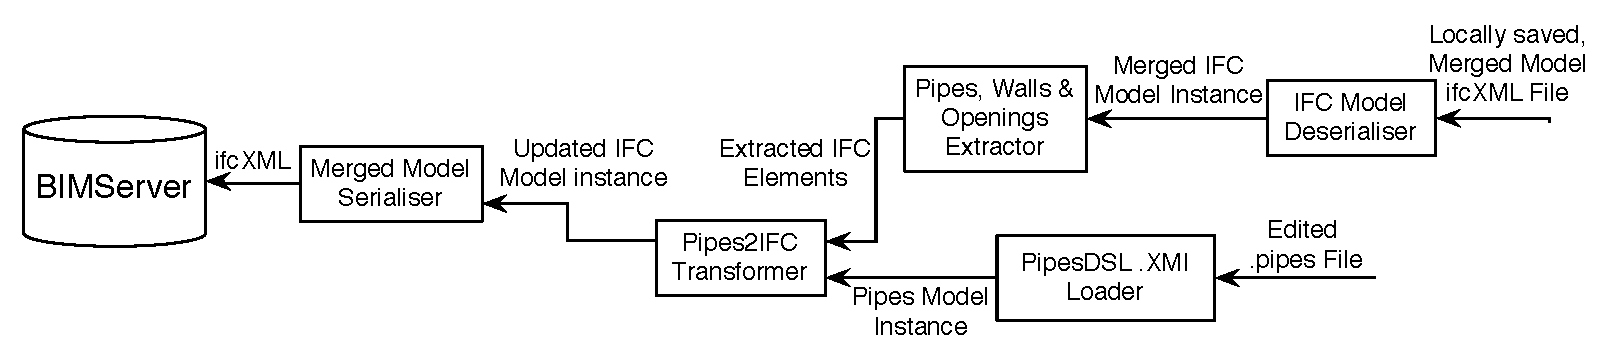
\includegraphics[width=120mm]{images/Pipes2IFC.pdf}
    \caption{Pipes DSL to IFC workflow}
    \label{fig:Pipes2IFCWorkflow}
\end{figure}

Clearly, most of the work in this workflow lies with the Main Model Updater, which uses a pattern match-like dispacth language feature of Xtend to elegantly update the java object graph of the extracted model. The routine runs through all elements in the Java object graph to update the corresponding Pipes DSL objects by looking at matching GUIDs. Only traversing an extract of the main model guarantees a better running time and still guarantees a correct update procedure, as the Pipes DSL does not allow any updates to elements outside of this extract anyway.
\subsubsection{Adding and Removing}
The setup not only supports updating the attributes of elements, it also allows the user to do structural changes on the model. The Main Model Updater looks for elements in the Pipes DSL object graph without a GUID to determine if a new element should be created in the IFC model. This feature allows the user to add missing openings for pipe segments and is therefore crucial for the usefulness of the end product. 
\paragraph{}
Likewise, if the updater fails to find an element in Pipes DSL object graph that corresponds to the existing one in the Java object graph it means the element has been deleted and that the Main Model Updater should take appropriate action to update references.

\subsection{Pipes DSL}
An example or two about the DSL and why it simplifies the work with the Pipes/Openings domain.













 %Describe the solution
%!TEX root = ./report.tex
\section{Evaluation}
Discussion of applicability of product. What should be done in order to make this project usable in a real world scenario?

Point out: It is not relevant to have evaluations of the usability of the textual language as it is only experimental. One would obviously make a visual editor if the product should be usable.

What were the challenges?
- Saving the subset back to the server after editing. Synchronization problem
- Using MPS: it is not a freetext editor. We would want to improve on this later. XText is not flexible enough for this purpose.



Threats to validity
Harrington point: We know that we only make changes to elements in our own domain in the IFC model and can show the correctness of the operations performed on these. But we have no way of showing that the open and save operations on the XML file work as intended. We say that our solution works correctly under the assumption that these methods work.
%!TEX root = ./report.tex

\section{Ideas for Future Projects}
\label{sec:plan_for_future_projects}
An overall goal of this pilot study was to increase the BIM knowledge of the environmentally concerned ITU research initiative, Energy Futures\footnote{For further information, see \url{http://energyfutures.itu.dk/}}. With this project as a point of departure, we have developed the following plan for future follow-up projects.

\subsection{Tools for Custom Open Source IFC Meta Model}
At the core of the prototype described in this paper is the IFC meta model. As described in Section \ref{subsec:requirements_evaluation}, our meta model generated from the ifcXML XSD has several problems, such as the lack of inverse relationships. Most of these problems could be solved by using a better, customised Ecore meta model, such as one made by Jim Steel\footnote{Jim Steel's model can be found at \url{http://www.emn.fr/z-info/atlanmod/index.php/Ecore#ifc2x3_0.1}} that we discovered late in the process. However, using this meta model would require writing serializers, which is not a trivial task. With Jim Steel's Ecore meta model as a starting point, one could a imagine an open source project in which a full-fledged serializer and deserializer for the IFC-EXPRESS language is developed, along with a revision of the meta model. This would enable future IFC developers to benefit from an independent toolset for working with IFC. These tools should support the dynamic nature of IFC, such that they are easily amended when updates to the IFC standard are released. Ideally, this Ecore meta model and the tools provided could serve as a common industry standard for working with IFC in EMF, making developers less dependent on proprietary tools.

% Study these papers:
%	"Feature-Based Survey of Model Transformation Approaches",
%	"The View Update Problem for XML",
%	"From model transformation to incremental bidirectional model synchronization" (very technical paper)
\subsection{Synchronisation}
    BIM projects should support distributed collaborative work on models. For example, we see that BIMserver is implemented with a notification system that can notify users when a model, or parts of a model, is changed. This indicates that if client software is to be useful in a real world scenario, it should be able to synchronize with the central model. As it was outside the scope of this project to require this kind of synchronization, the final solution is rather static compared to what is desirable. Currently no real synchronization takes place. We update the extracted sub-set of the source model with the PipesDSL that has been edited. This resembles source-incrementality (\cite{czarnecki06} pp. 14), and will be important for fast synchronization with a big source model like IFC. Still we do this without considering that the source model could have changed. Also, the workflow from IFC to pipes, will always create, or overwrite, the target model without considering a scenario where an existing target model is being edited. To be able to approach the synchronization problem, we believe it should be possible to expand on the current transformation implemented with Xtend. To be able to track changes and examine models before synchronization, we could use traceability\cite{czarnecki06} to record what rules have been applied to the elements in the models. Xtend offers a tracing package\cite{xtendtrace} for this. We imagine a project called something like $Synchronization with IFC$ that could be based on our work, and investigate how a simple domain like PipesDSL can handle synchronization with a source model, possibly at BIMServer. We think this would be a challenging and interesting project, that addresses an open problem in MDD.

\paragraph{MVD}

\paragraph{DSL}

\subsection{Structural Changes}
Handling structural changes in the source model is challenging. With PipesDSL we simply insert new elements without validating the source model, which is too naive to work in real-world scenarios. For example, when inserting a new pipe, we can imagine that a cost or energy object would need to reference this newly inserted object. Our project has allowed that we might break such constraints in the source model, as it is not clear how dependencies and constraints should be checked. We think a domain specific software, that can make it easy to define constraints for the IFC model, and do automatic validation of the model here upon, could be interesting. A project with something like an $IFC Validator$ could provide a DSL for defining constraints within a domain like pipes and walls, and subsequently validate an IFC instance based on these constraints. Our work could be used as test software for performing the model transformations, and the $IFC Validator$ should then be able to indicate what constraints have been violated by the structural change. The project would require a clear definition of the target domain and a study of relevant real world models.

%!TEX root = ./report.tex
\section{Related Work}
\label{sec:related_work}
The problem of partial model editing and synchronization is a common one. Here we present a couple of closely related projects as well as other important alternative approaches and resources.

%A Graphical User Interface for Handling IFC Partial Model exchange
Nour argues that the exchange of partial models is one of the central challenges of widespread use of a central model for BIM, mainly IFC\,\cite{nour08}. Although we do not adopt his idea of end-user filtering through the use of MVD, our approach does incorporate software filtering for defining a working subset of IFC.

%BSPro COM-Server -- interoperability between software tools using industrial foundation classes
Karola et al. describe an early solution to the partial model extraction and update problem implemented as middleware. The BSPro COM-Server bridges various existing tools, each requiring a specific subset of IFC, making interoperability possible \cite{karola02}.

%Embedded Software Development with Projectional Language Workbenches
%PrEdE: a Projectional Editor for the Eclipse Modeling Framework
An alternative to our approach, is projectional editing. As specified by Tomasetti et al.\,\cite{tomasetti11}, projectional editors operate directly on the model, and thus no model synchronisation is involved. An example of a projectional editor is Jetbrains MPS.\footnote{Jetbrains MPS can be found at \url{http://www.jetbrains.com/mps/}} This approach trades loss of notational flexibility for a guarantee of model consistency\,\cite{conf/models/Voelter10}. Consequently, in order to bring the notation as close to the domain as possible, a projectional editor was not desirable for our solution.

%Towards a Framework for a Domain Specific Open Query Language for Building Information Models
Another way to derive and edit subsets of an IFC model is through the use of the BIM Query Language\,\cite{mazairac10}. This language provides access to IFC models via an SQL-like syntax. The queried model is stored on a BIMServer. While the BIM Query Language does provide much more flexibility in terms of extraction and editing of IFC data when compared to the prototype presented in this paper, it does not provide the same closeness to the chosen subdomain.

%From model transformation to incremental bidirectional model synchronization
%The View Update Problem for XML
Staworko et al. define and discuss the view-update problem for instances where both the view and the source are XML documents\,\cite{staworko10}. Any Ecore model, i.e. also the Pipes DSL model, can be converted to XMI, thus making the formalisations of both the view-update problem and its solutions are very relevant for the future work on our synchronisation logic.

%Feature-Based Survey of Model Transformation Approaches
The model transformations used in our solution has mainly been realised through the direct manipulation approach described by Czarnecki et al.\,\cite{czarnecki06}, facilitated by the dispatch method feature of Xtend and the clarity of the MWE2.

%TODO reference this paper somewhere in the paper
%Design guidelines for DSLs
As the design of the concrete syntax for the presented DSL has been a minor aspect of our solution, it is far from perfect. The guidelines for DSL design presented by Karsai et al.\,\cite{karsai09} has been used as the basis for the preliminary design of the DSL, and further work in this direction will most likely benefit from the guidelines.






%TODO: include a reference to this somewhere in the report: Industry Foundation Classes And Interoperable Commercial Software In Support Of Design Of Energy-Efficient Buildings


%!TEX root = ./report.tex
\section{Conclusion}
\label{sec:conclusion}
As evaluated in Section \ref{sec:evaluation}, the requirements for a partial editor prototype set forward in Section \ref{subsec:requirements}, have been met. Furthermore, the correctness of the output has been verified with an account for threats to validity. Finally, a plan for future BIM-related projects has been presented, assisting the ITU research initiative, Energy Futures, in increasing their understanding of this problem domain. We conclude that editing on a subset of an IFC model is feasible using modern modelling tools.

\subsubsection{Acknowledgements} Special thanks to associate professor at Aalborg University Kaj Jørgensen for providing example IFC models as well as overall guidance in selecting a fitting IFC domain for our project. Furthermore, we thank construction management student at Copenhagen School of Design and Technology, Mathias Demant, for providing example IFC models mainly used for testing.
%!TEX root = ./report.tex
\bibliography{report}

%% Old bibliography
% %
% % ---- Bibliography ----
% %
% \begin{thebibliography}{99}
% %

% \bibitem[3]{2mich:tar}
% Michalek, R., Tarantello, G.:
% Subharmonic solutions with prescribed minimal
% period for nonautonomous Hamiltonian systems.
% J. Diff. Eq. 72, 28--55 (1988)

% \bibitem[4]{2tar}
% Tarantello, G.:
% Subharmonic solutions for Hamiltonian
% systems via a $\bbbz_{p}$ pseudoindex theory.
% Annali di Matematica Pura (to appear)

% \bibitem[5]{2rab}
% Rabinowitz, P.:
% On subharmonic solutions of a Hamiltonian system.
% Comm. Pure Appl. Math. 33, 609--633 (1980)


% \end{thebibliography}
%!TEX root = ./report.tex
\newpage
\appendix
\section{Results of Black Box Tests}
\label{app:blackboxtests}
%Test
%VERY IMPORTANT TODO: mention which test buildings were used and where they can be found.
\subsection{Cases:}
For these tests, we have several cases: One of them is a subset of a real IFC model, provided by Kaj J\o rgensen. The rest have been created by Mathias Demant for our testing, and do not represent any real buildings. The files can be found in Prototype/Model2ModelWorkflows/NanoLabBuilding/ on the attached medium. The results can be seen in Figures \ref{fig:test1}, \ref{fig:test2}, \ref{fig:test3}, and \ref{fig:test4}.
\subsection{Tests:}
For each case, we will perform the following tests between the two MWE2 workflows:
\subsubsection{Test 1:}
Modifying the metadata (name, description) for one of each of the three product types (wall, opening, flow segment).
\textbf{Expected result:} The output IFC model differs from the input IFC model in that it has altered metadata (name, description).
\subsubsection{Test 2:}
Modifying the placement of one of each of the three products types.
\textbf{Expected result:} A new IFCLocalPlacement object now exists in the IFC output model with the modified metadata. 
\subsubsection{Test 3:}
Modifying the list of walls in a opening element
\textbf{Expected result:} A new IFCRelVoidElement is present in the output IFC model, compared to the input mode, linking the wall and opening.
\subsubsection{Test 4:}
Deleting one Pipe.
\textbf{Expected result:} The output IFC model no longer contains the deleted flow segment. Any created orphans should be garbage collected.
\subsubsection{Test 5:}
Adding one opening.
\textbf{Expected result:} The output IFC model should now contain the created opening, along with any new objects referenced by the opening (LocalPlacement, Axis2Placement3d)
\subsubsection{Test 6:}
Adding one opening, deleting one flow segment, and modifying metadata for one wall.
\textbf{Expected result:} The output IFC model should now contain the created opening (along with referenced objects), the flow segment should be deleted (along with orphans), and the metadata for the wall should be updated.
\begin{figure}[ht]
    \centering
        \centerline{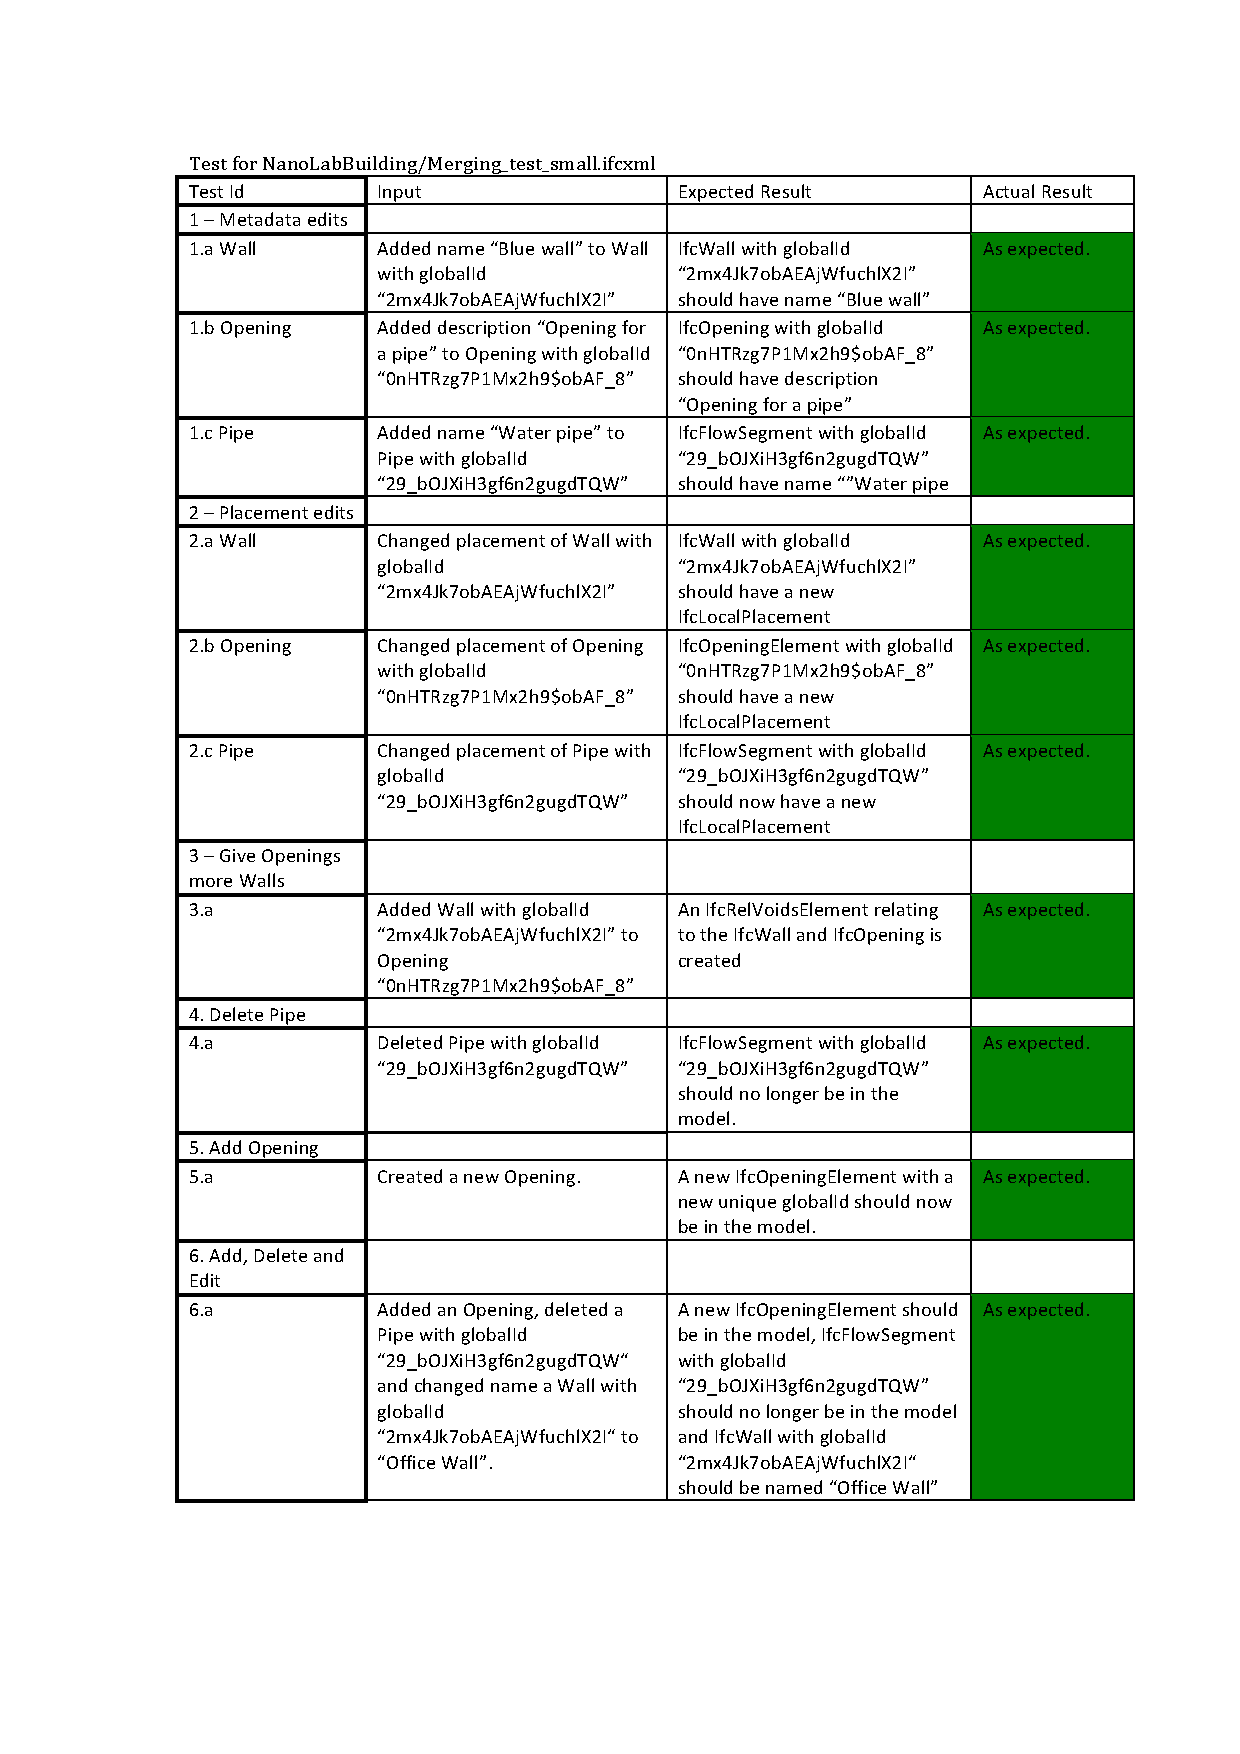
\includegraphics[width=150mm]{images/Test1.pdf}}
    \caption{}
    \label{fig:test1}
\end{figure}
\begin{figure}[ht]
    \centering
        \centerline{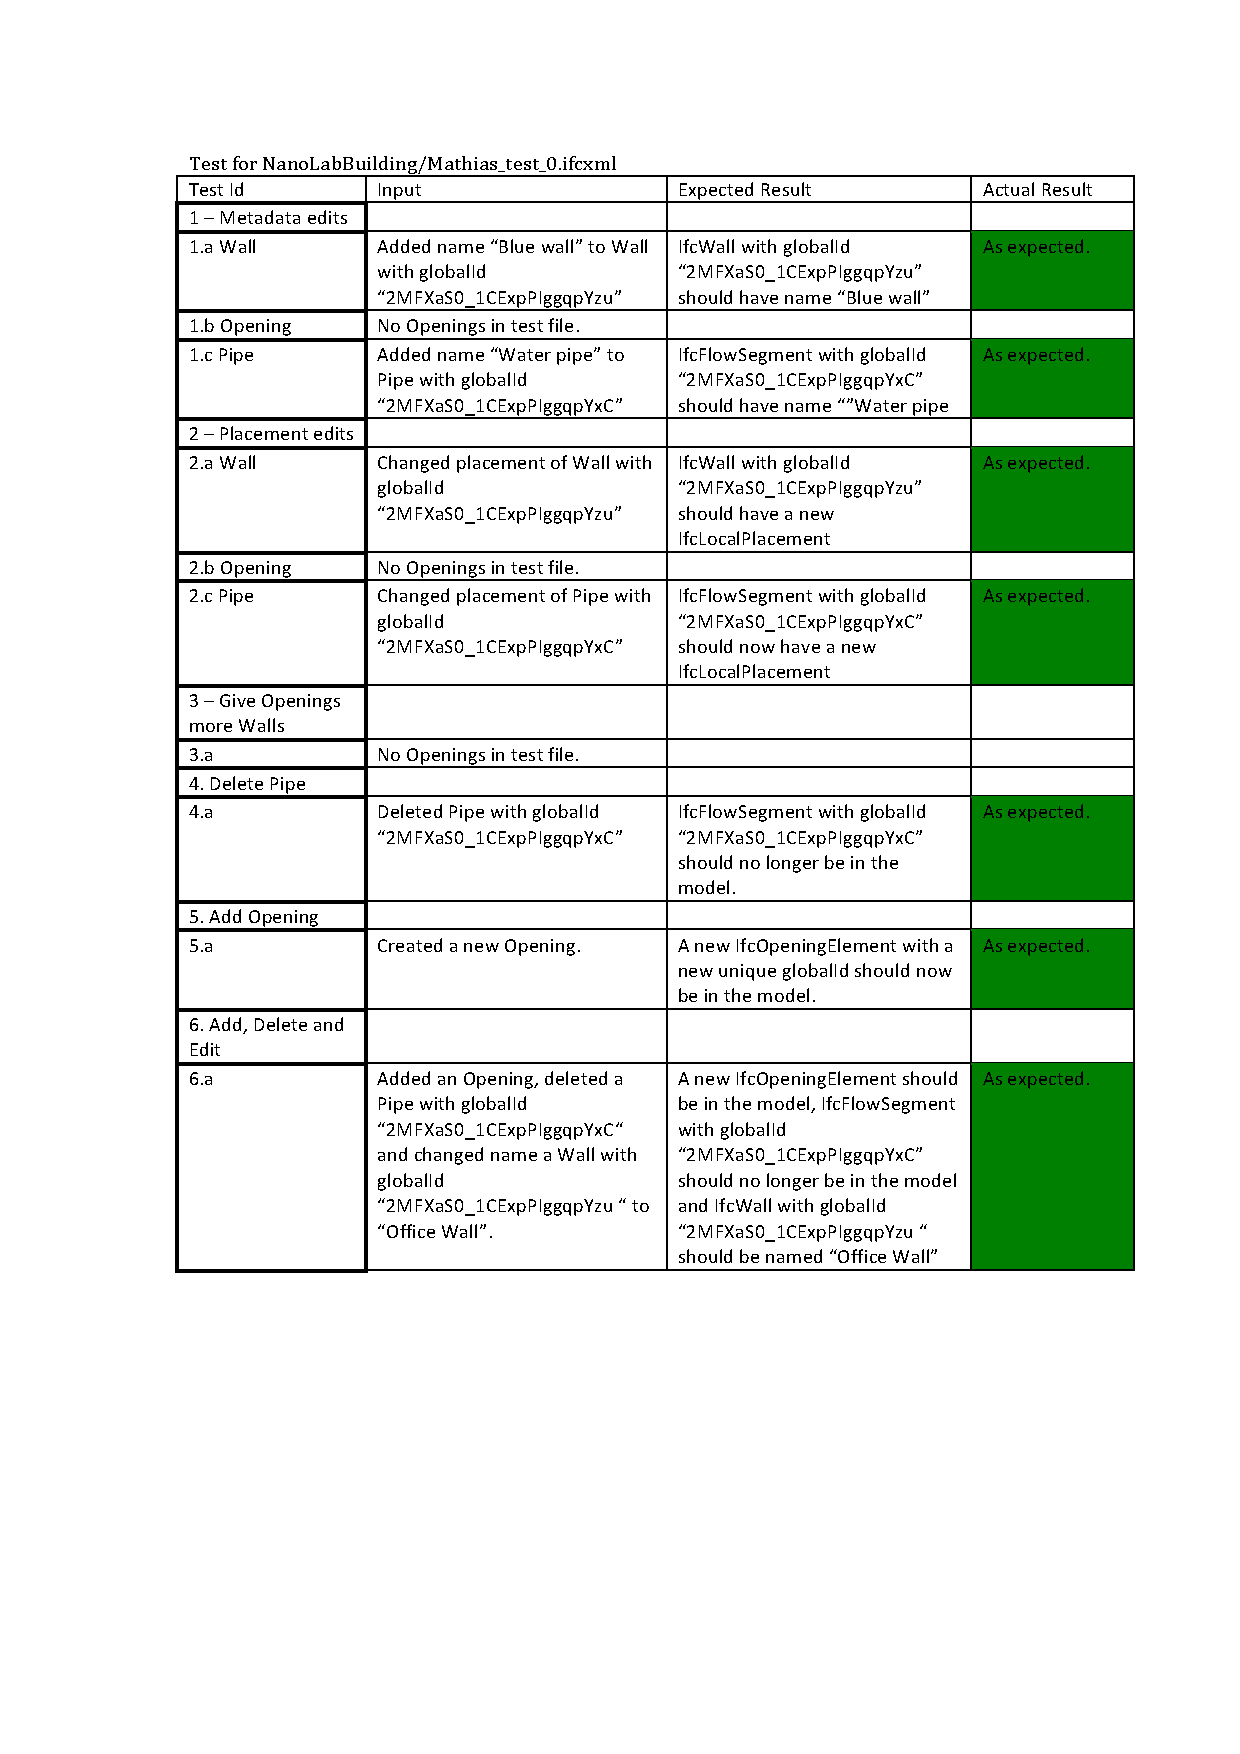
\includegraphics[width=150mm]{images/Test2.pdf}}
    \caption{}
    \label{fig:test2}
\end{figure}
\begin{figure}[ht]
    \centering
        \centerline{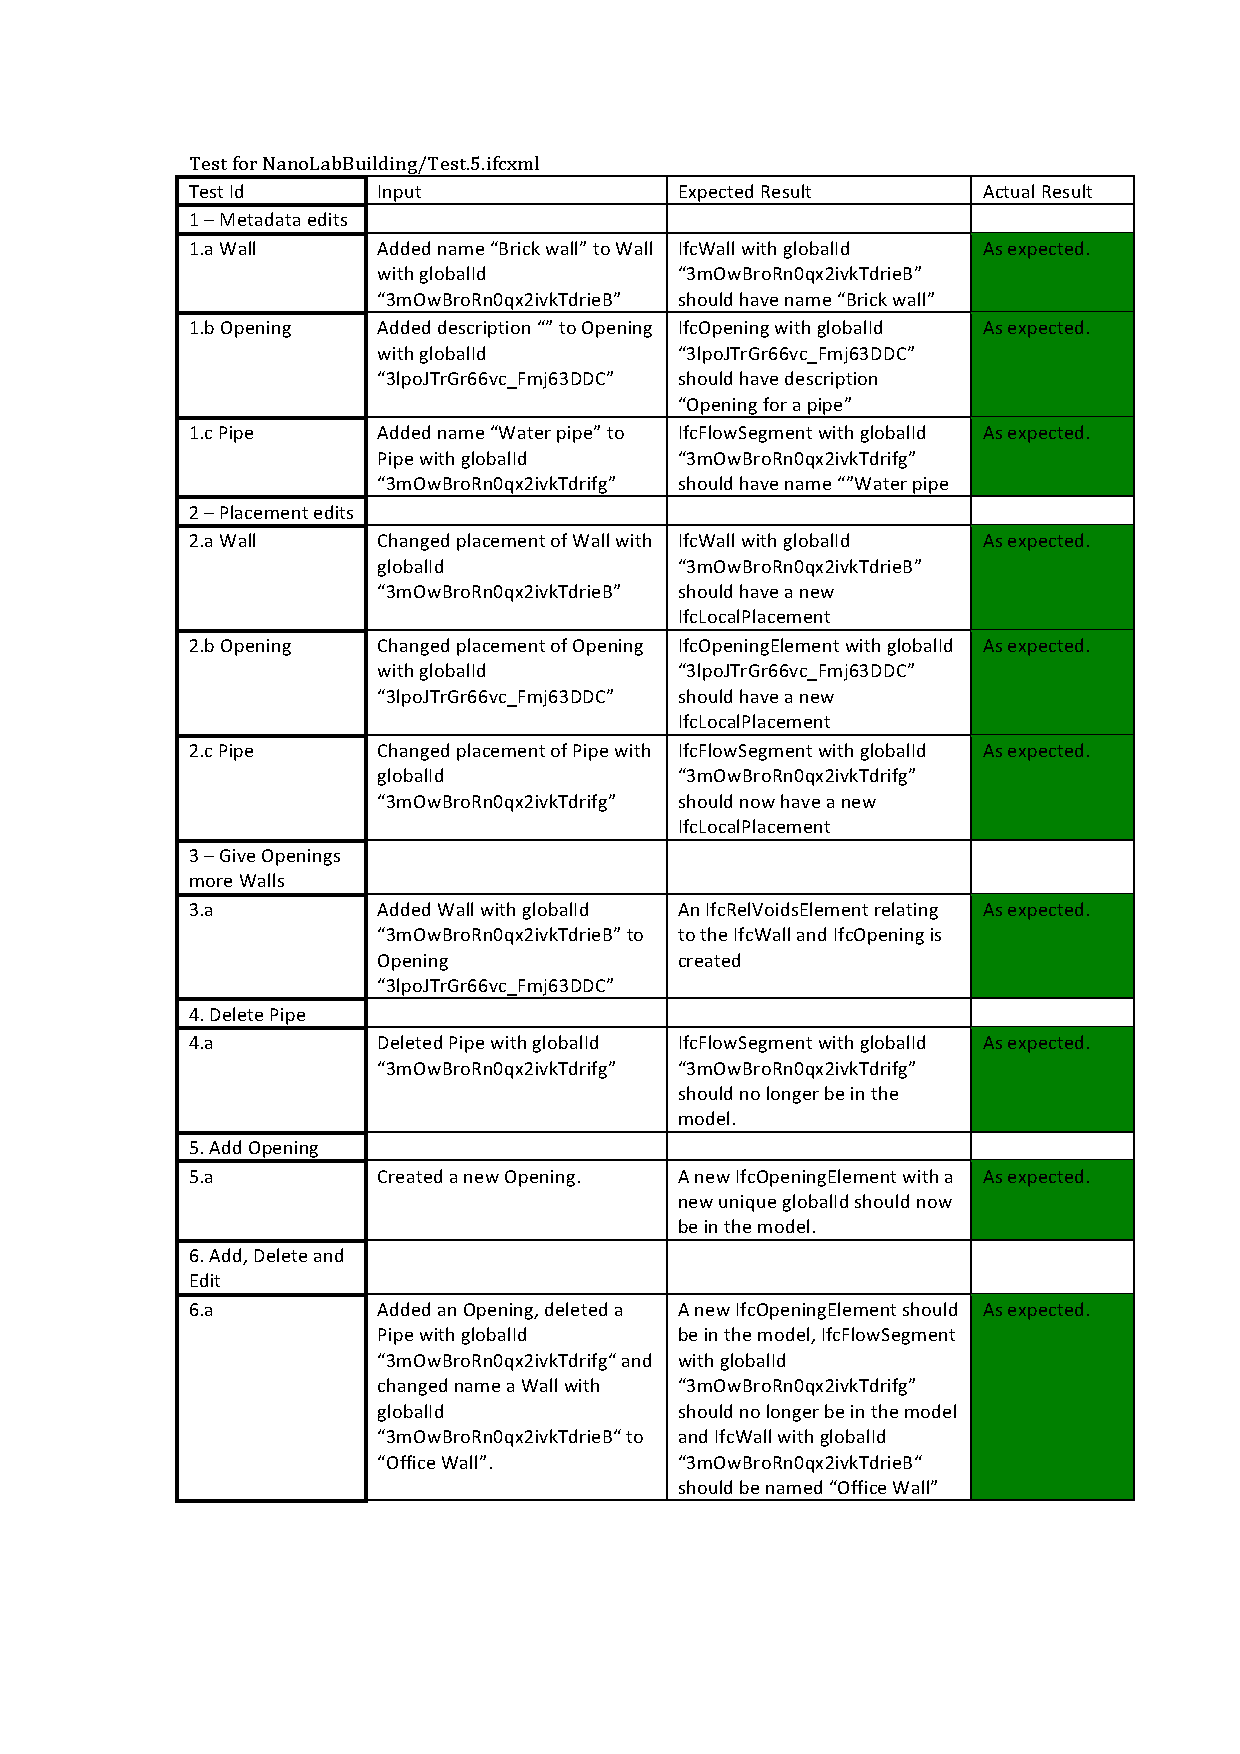
\includegraphics[width=150mm]{images/Test3.pdf}}
    \caption{}
    \label{fig:test3}
\end{figure}
\begin{figure}[ht]
    \centering
        \centerline{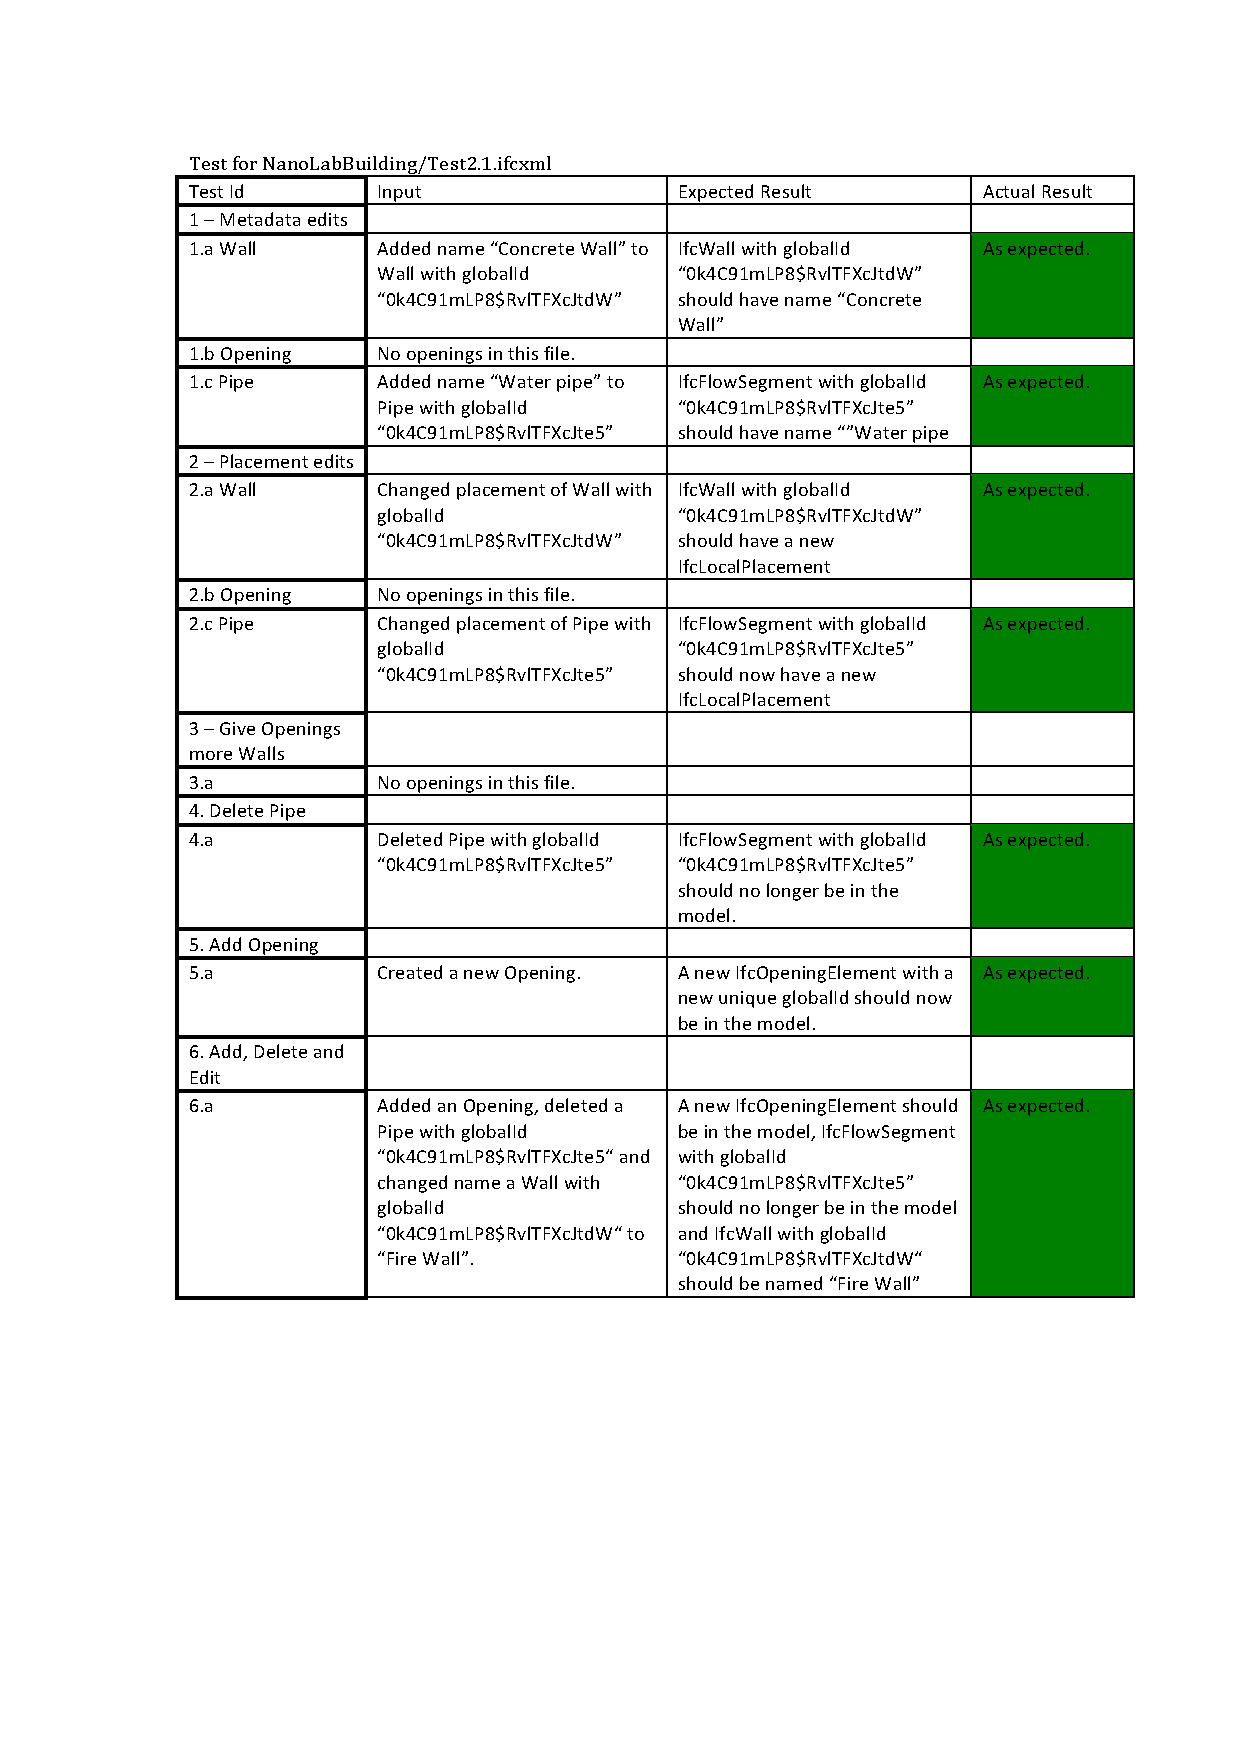
\includegraphics[width=150mm]{images/Test4.pdf}}
    \caption{}
    \label{fig:test4}
\end{figure}


\section{Automated Tests}
\label{app:automatedtests}
The workflow components used for tests can be found in the Eclipse project under: Model2ModelWorkflows/src/tests. These components work as a part of two test workflows similar to the ones used in the actual prototype. The only difference is that test components have been inserted after extraction and transformation components. The IFC2Pipes.mwe2 workflow is thus tested by the IFC2PipesTest.mwe2 workflow and the Pipes2IFC.mwe2 workflow is tested by the Pipes2IFCTest.mwe2 workflow.

\subsubsection{Testing Element Extraction}
The TestIFCExtractor workflow component verifies that the extraction process executed with a correct result. On any input building it checks that the number of extracted IfcProducts correspons to the number of products that should be extracted by looking directly at the ifcXML. For each of the extracted product elements it tests for a valid GUID and ID. On all input models of Appendix \ref{app:blackboxtests} the test passes.

\subsubsection{Testing IFC to Pipes Model Transformation}
The following consistency verification between elements in the IFC and Pipes models are carried out:

\begin{itemize}
	\item IfcFlowSegment <-> FlowSegment
	\item IfcOpening <-> Opening
	\item IfcWall <-> Wall
	\item IfcLocalPlacement <-> LocalPlacement
	\item IfcAxis2Placement3d <-> Axis2Placement3D
	\item IfcDirection <-> Direction
\end{itemize}

By going through all extracted IFC products after the model to model transformation and comparing them to the elements of the Pipes model, the TestTransformers test component automates transformation testing of the subdomain. All consistency tests on all input buildings from Appendix \ref{app:blackboxtests} pass the tests.

\subsubsection{Testing Pipes to IFC Update Routine}
The TestTransformer test component is used for the purpose of testing the Pipes to IFC Update Routine as well. The same consistency checks are performed after the Pipes2IFCTransformer, which performs this routine. The same element relations, as above, are tested. All consistency tests on all input buildings from Appendix \ref{app:blackboxtests} pass the tests.








\end{document}









